\documentclass[10pt]{article}

\usepackage[margin=1in]{geometry}
\usepackage{amsmath,amssymb}
\usepackage{graphicx}
\usepackage{booktabs}
\usepackage{hyperref}
\usepackage{microtype}
\usepackage{parskip}
\usepackage{enumitem}
\usepackage{caption}
\usepackage{float}
\usepackage{xcolor}
\usepackage{array}
\usepackage{multirow}
\usepackage{subcaption}

\hypersetup{
    colorlinks=true,
    linkcolor=blue!60!black,
    citecolor=blue!60!black,
    urlcolor=blue!60!black,
}

\title{%
    \large\textbf{Injecting Epipolar Geometry into MatchFormer:}\\
    \large\textbf{Inference-Time Constraints and Supervised Fine-Tuning}
}
\author{Siddharth Raj}
\date{March 2026}

\begin{document}

\maketitle

%─────────────────────────────────────────────────────────────────────────────
\begin{abstract}
We investigate two strategies for improving the geometric quality of matches produced by MatchFormer, a transformer-based image matcher. First, we inject a soft epipolar mask into the coarse confidence matrix at inference time—a training-free approach that biases match selection toward geometrically plausible regions. Second, we fine-tune the model weights with epipolar-aware supervision on ScanNet. Evaluated on 100 ScanNet indoor image pairs, inference-time epipolar injection reduces mean reprojection error by \textbf{65\%} (92.67\,$\to$\,32.77\,px) while preserving match density. Fine-tuning achieves a \textbf{93--94\% reduction} in mean error (92.67\,$\to$\,5.95\,px) and a \textbf{546$\times$ improvement} in Precision@3px (0.04\%\,$\to$\,21.83\%) at a confidence threshold of 0.10, while maintaining 436 matches per pair—sufficient for downstream pose estimation.
\end{abstract}

%─────────────────────────────────────────────────────────────────────────────
\section{Introduction}

Modern image matching pipelines for 3D reconstruction, visual localization, and SLAM rely on dense or semi-dense feature matchers. MatchFormer~\cite{matchformer} interleaves self- and cross-attention across multiple scales, producing correspondences without explicit descriptor computation. While effective, the model is trained purely for feature similarity and has no explicit awareness of camera geometry at inference time.

Epipolar geometry provides a hard constraint on valid correspondences: a point $p_i$ in image~0 must correspond to a point $p_j$ in image~1 lying on the epipolar line $l'_j = F p_i$, where $F$ is the fundamental matrix derived from known poses and intrinsics. This constraint can be exploited in two complementary ways:

\begin{enumerate}[leftmargin=*,itemsep=2pt]
    \item \textbf{Inference-time masking.} Multiply a soft epipolar mask into the confidence matrix without changing model weights. No training required; poses must be available at inference time.
    \item \textbf{Supervised fine-tuning.} Apply the epipolar mask during training as part of a focal loss, so the model internalizes the geometric prior. No poses required at inference time.
\end{enumerate}

This report evaluates both approaches quantitatively on ScanNet \texttt{scene0000\_00}.

%─────────────────────────────────────────────────────────────────────────────
\section{Background}

\subsection{MatchFormer}

MatchFormer (Lite-LA variant) uses a hierarchical linear-attention backbone with four stages. Self-attention and cross-attention alternate at each stage, allowing image features to interact progressively. The coarse matching module computes a joint confidence matrix:
\begin{equation}
    C = \operatorname{softmax}(S/T)_{\text{row}} \;\odot\; \operatorname{softmax}(S/T)_{\text{col}}
\end{equation}
where $S_{ij} = \langle f_i^{(0)}, f_j^{(1)} \rangle / \sqrt{d}$ is the feature similarity and $T$ is a learned temperature. A match $(i,j)$ is accepted when $C_{ij} > \tau_{\text{thr}}$ (default $\tau_{\text{thr}} = 0.20$), followed by a fine-level sub-pixel refinement step.

\subsection{Epipolar Geometry and Coordinate Conventions}

Given camera poses and intrinsic matrix $K$, the fundamental matrix $F$ maps a point $p_0 = (u, v, 1)^\top$ in image~0 to an epipolar line $l' = F p_0$ in image~1. The point-to-line distance for a candidate match $p_1$ is:
\begin{equation}
    d(p_1, l') = \frac{|{l'}^\top p_1|}{\sqrt{l_1'^2 + l_2'^2}}
\end{equation}

ScanNet stores poses in \textbf{camera-to-world / OpenGL convention} ($+Y$ up, $-Z$ forward). Converting to OpenCV convention ($+Y$ down, $+Z$ forward) requires:
\begin{equation}
    T_{\text{cv}} = T_{\text{gl}} \cdot \begin{bmatrix} 1 & 0 & 0 & 0 \\ 0 & -1 & 0 & 0 \\ 0 & 0 & -1 & 0 \\ 0 & 0 & 0 & 1 \end{bmatrix}
\end{equation}
The relative pose $T_{12} = T_{2,\text{cv}}^{-1} T_{1,\text{cv}}$ yields the essential matrix $E = [t]_\times R$ and fundamental matrix $F = K^{-\top} E K^{-1}$. This was validated against OpenCV's \texttt{findFundamentalMat} with sub-pixel agreement ($<10^{-6}$\,px error).

%─────────────────────────────────────────────────────────────────────────────
\section{Dataset}

\subsection{ScanNet}

We use \textbf{ScanNet}~\cite{scannet}, a large-scale RGB-D dataset of indoor scenes captured with a structured-light depth sensor. ScanNet provides per-frame color images, depth maps, camera-to-world poses, and camera intrinsics, making it well-suited for evaluating geometric matching methods where ground-truth reprojection can be computed exactly.

\subsection{Scene Selection and Download}

We downloaded 11 scenes spanning a variety of indoor environments (living rooms, bedrooms, bathrooms, corridors):

\begin{table}[H]
\centering
\caption{Downloaded ScanNet scenes and frame counts.}
\label{tab:scenes}
\small
\begin{tabular}{lc}
\toprule
\textbf{Scene} & \textbf{Frames} \\
\midrule
scene0000\_00 & 5,578 \\
scene0001\_00 & 1,544 \\
scene0002\_00 & 5,193 \\
scene0003\_00 & 1,736 \\
scene0004\_00 &   929 \\
scene0005\_00 & 1,159 \\
scene0006\_00 & 2,160 \\
scene0007\_00 & 1,041 \\
scene0008\_00 & 1,038 \\
scene0009\_00 &   980 \\
scene0010\_00 & 2,513 \\
\midrule
\textbf{Total} & \textbf{23,871} \\
\bottomrule
\end{tabular}
\end{table}

Scenes were downloaded from the official ScanNet server as binary \texttt{.sens} files using the ScanNet download script with the \texttt{--type .sens} flag, targeting individual scenes via \texttt{--id scene\{XXXX\}\_00}.

\subsection{Extraction Pipeline}

ScanNet \texttt{.sens} files use a custom binary format (version 4) that is not directly readable by standard libraries. We wrote a custom extraction script (\texttt{extract\_scannet.py}) to parse these files locally. The binary header layout is:

\begin{itemize}[leftmargin=*,itemsep=1pt]
    \item \texttt{version} (uint32, 4 B)
    \item \texttt{strlen} (uint64, 8 B) + \texttt{scene\_name} (\texttt{strlen} bytes)
    \item Four fixed $4{\times}4$ float32 matrices (256 B total): color intrinsics, color extrinsic, depth intrinsics, depth extrinsic
    \item \texttt{color\_compression}, \texttt{depth\_compression} (int32, 4 B each)
    \item \texttt{color\_width}, \texttt{color\_height}, \texttt{depth\_width}, \texttt{depth\_height} (uint32, 4 B each)
    \item \texttt{depth\_shift} (float32, 4 B), \texttt{num\_frames} (uint64, 8 B)
\end{itemize}

Each frame stores: camera-to-world pose (64 B), timestamps (16 B), compressed color and depth byte counts (16 B), followed by the raw JPEG-compressed color data and zlib-compressed depth data.

The extraction script exports four subdirectories per scene:
\begin{itemize}[leftmargin=*,itemsep=1pt]
    \item \texttt{color/} — JPEG frames at native resolution ($1296 \times 968$), resized to $640 \times 480$ during training
    \item \texttt{depth/} — 16-bit PNG depth maps ($640 \times 480$), depth in millimetres with scale factor 1000
    \item \texttt{pose/} — per-frame $4{\times}4$ camera-to-world matrices as \texttt{.txt} files
    \item \texttt{intrinsic/} — \texttt{intrinsic\_depth.txt} containing the $4{\times}4$ depth intrinsic matrix $K$
\end{itemize}

After extraction the \texttt{.sens} file is automatically deleted to conserve disk space. The extracted data was then uploaded to Google Drive for use in Colab training.

\subsection{Training Pairs}

Image pairs are constructed by pairing frames separated by a fixed \textbf{frame gap of 20}, giving moderate viewpoint change with sufficient overlap for meaningful supervision. With 23,871 total frames across 11 scenes, this yields \textbf{23,651 pairs} for training. Pairs are constructed within scenes only — cross-scene pairs are not used, as camera poses are not defined across scenes.

For evaluation, 100 pairs are drawn from \texttt{scene0000\_00} using the same 20-frame gap.

\subsection{Code and Reproducibility}

All code — including the \texttt{.sens} extraction script, training pipeline, benchmark scripts, and analysis notebooks — is available at:

\begin{center}
\url{https://github.com/sid-raj-uc/match-former}
\end{center}

Key files are listed in Section~\ref{sec:impl}.

%─────────────────────────────────────────────────────────────────────────────
\section{Method}

\subsection{Soft Epipolar Mask}

We define a soft epipolar mask at coarse feature resolution as:
\begin{equation}
    M_{ij} = \exp\!\left(-\frac{d\bigl(p_i^{(0)},\, l'_j\bigr)}{\tau}\right)
\end{equation}
where $\tau$ controls the constraint bandwidth. This mask is multiplied into the confidence matrix before match selection:
\begin{equation}
    \hat{C} = C \odot M
\end{equation}
At stride~8, the feature grid is $60 \times 80 = 4800$ points per image, so the distance matrix $M \in \mathbb{R}^{4800 \times 4800}$ is materialized in blocks of 512 rows to avoid GPU out-of-memory.

\subsection{Inference-Time Injection}

For evaluation without fine-tuning, we monkey-patch \texttt{CoarseMatching.forward} to compute and inject the mask per image pair using ground-truth poses. Model weights are left unchanged.

\subsection{Supervised Fine-Tuning}

\paragraph{Dataset.} ScanNet \texttt{scene0000\_00}, 5,578 frames $\to$ 5,556 consecutive pairs at a 20-frame gap. A 90/10 train/val split was used, yielding approximately 5,000 training pairs.

\paragraph{Loss function.} The total loss combines a coarse-level focal loss and a fine-level L2 offset loss:
\begin{equation}
    \mathcal{L} = \lambda_c \cdot \mathcal{L}_{\text{focal}} + \lambda_f \cdot \mathcal{L}_{\text{fine}}
\end{equation}

The focal loss~\cite{focalloss} operates on the epipolar-masked confidence matrix $\hat{C}$ with binary GT match labels derived from depth-projected correspondences:
\begin{align}
    \mathcal{L}_{\text{focal}} = -\frac{1}{|\mathcal{P}|} \sum_{i,j} \Big[
        &y_{ij} \cdot \alpha (1 - \hat{C}_{ij})^\gamma \log \hat{C}_{ij} \nonumber \\
        + &(1-y_{ij}) \cdot (1-\alpha) \hat{C}_{ij}^\gamma \log(1 - \hat{C}_{ij}) \Big]
\end{align}
with $\alpha = 0.25$, $\gamma = 2.0$, $\lambda_c = 1.0$, $\lambda_f = 0.5$.

The fine loss applies an uncertainty-weighted L2 penalty on the predicted sub-pixel offset for GT-matched positions:
\begin{equation}
    \mathcal{L}_{\text{fine}} = \frac{1}{N} \sum_{k \in \text{GT}} \frac{\|\hat{\delta}_k\|^2}{\hat{\sigma}_k}
\end{equation}
where $\hat{\sigma}_k$ is the model's predicted standard deviation for match $k$.

\paragraph{Training setup.} Table~\ref{tab:training} summarizes the hyperparameters.

\begin{table}[H]
\centering
\caption{Fine-tuning hyperparameters.}
\label{tab:training}
\small
\begin{tabular}{ll}
\toprule
\textbf{Hyperparameter} & \textbf{Value} \\
\midrule
Base checkpoint         & \texttt{indoor-lite-LA.ckpt} \\
Training steps          & 10,000 \\
Batch size              & 2 \\
Learning rate           & $10^{-4}$ (cosine $\to 10^{-6}$) \\
Optimizer               & AdamW, wd $= 10^{-4}$ \\
Epipolar $\tau$ (train) & 10.0 \\
Gradient clip           & 1.0 \\
Platform                & Google Colab, Tesla T4 \\
\bottomrule
\end{tabular}
\end{table}

%─────────────────────────────────────────────────────────────────────────────
\section{Evaluation Protocol}

\subsection{Dataset and Pairs}
100 image pairs from ScanNet \texttt{scene0000\_00}, separated by 20 frames (moderate overlap, non-trivial viewpoint change). All images are resized to $480 \times 640$ px.

\subsection{Ground-Truth Reprojection Metric}

For each predicted match $(p_0, \hat{p}_1)$:
\begin{enumerate}[leftmargin=*,itemsep=1pt]
    \item Sample depth $z$ at $p_0$ from the aligned depth map.
    \item Unproject: $P = K^{-1}[p_0; 1] \cdot z$.
    \item Transform: $P' = T_{12}[P; 1]$.
    \item Project: $p_1^* = K P' / P'_z$.
    \item Error: $e = \|\hat{p}_1 - p_1^*\|_2$.
\end{enumerate}
Matches with $z \leq 0.1$\,m, $z > 10$\,m, or projected GT outside the image are excluded. Pairs with zero valid matches are skipped.

\subsection{Metrics}

\begin{itemize}[leftmargin=*,itemsep=1pt]
    \item \textbf{Mean GT Error (px):} Average reprojection error over valid matches.
    \item \textbf{P@3px:} Fraction of valid matches with error $< 3$\,px.
    \item \textbf{P@5px:} Fraction of valid matches with error $< 5$\,px.
    \item \textbf{Avg Matches:} Average depth-verified matches per pair.
\end{itemize}

%─────────────────────────────────────────────────────────────────────────────
\section{Results}

\subsection{Baseline: Vanilla MatchFormer}

\begin{table}[H]
\centering
\caption{Vanilla MatchFormer baseline (thr\,=\,0.20).}
\label{tab:vanilla}
\small
\begin{tabular}{lc}
\toprule
\textbf{Metric} & \textbf{Value} \\
\midrule
Mean GT Error & 92.67\,px \\
P@3px         & 0.04\%    \\
P@5px         & 0.09\%    \\
Avg Matches   & 2,567     \\
\bottomrule
\end{tabular}
\end{table}

The vanilla model produces dense matches but most are geometrically incorrect under the strict reprojection metric—expected, as the model was never trained with geometric supervision.

\subsection{Inference-Time Epipolar Injection ($\tau$ Sweep)}

Table~\ref{tab:tau} shows results for varying $\tau$ on the original, unmodified weights.

\begin{table}[H]
\centering
\caption{Vanilla weights with inference-time epipolar mask at varying $\tau$.}
\label{tab:tau}
\small
\setlength{\tabcolsep}{4pt}
\begin{tabular}{ccccc}
\toprule
$\tau$ & Error (px) & Error $\downarrow$ & P@3px & Avg Matches \\
\midrule
50.0       & 59.90  & $-35\%$ & 0.04\% & 1,187 \\
20.0       & 40.49  & $-56\%$ & 0.05\% & 577   \\
10.0       & 36.26  & $-61\%$ & 0.07\% & 300   \\
5.0        & 34.24  & $-63\%$ & 0.14\% & 147   \\
\textbf{2.0} & \textbf{32.77} & $\mathbf{-65\%}$ & \textbf{0.49\%} & \textbf{54} \\
\bottomrule
\end{tabular}
\end{table}

Tightening $\tau$ monotonically improves error and precision at the cost of match count. At $\tau = 2$, mean error drops 65\% and P@3px improves $12\times$, but only 54 matches remain per pair.

\subsection{Fine-Tuned Model: Threshold Sweep}

After fine-tuning, the model's confidence score distribution shifts downward. Table~\ref{tab:thr} sweeps the matching threshold $\tau_{\text{thr}}$.

\begin{table}[H]
\centering
\caption{Fine-tuned model (\texttt{last.ckpt}) at varying confidence thresholds.}
\label{tab:thr}
\small
\setlength{\tabcolsep}{4pt}
\begin{tabular}{ccccc}
\toprule
thr & Error (px) & P@3px & P@5px & Avg Matches \\
\midrule
0.20       & 3.33\,px & 20.38\% & 33.60\% & 2     \\
\textbf{0.10} & \textbf{5.95\,px} & \textbf{21.83\%} & \textbf{46.90\%} & \textbf{436} \\
0.05       & 6.42\,px & 18.03\% & 41.36\% & 1,994 \\
0.02       & 6.78\,px & 16.45\% & 38.30\% & 2,809 \\
0.01       & 6.85\,px & 16.23\% & 37.87\% & 2,894 \\
\bottomrule
\end{tabular}
\end{table}

\textbf{thr\,=\,0.10 is the optimal operating point}: best P@3px (21.83\%) and P@5px (46.90\%) with 436 matches per pair—well above the RANSAC minimum.

\subsection{Full Comparison}

Table~\ref{tab:full} summarizes all model variants at their best operating points.

\begin{table}[H]
\centering
\caption{Full comparison across all model variants.}
\label{tab:full}
\small
\setlength{\tabcolsep}{3.5pt}
\begin{tabular}{lcccc}
\toprule
\textbf{Model Variant} & \textbf{Error} & \textbf{P@3px} & \textbf{P@5px} & \textbf{Matches} \\
\midrule
Vanilla (thr=0.20)          & 92.67\,px & 0.04\%  & 0.09\%  & 2,567 \\
Vanilla + Epi.\ ($\tau$=10) & 36.26\,px & 0.07\%  & 0.17\%  & 300   \\
Vanilla + Epi.\ ($\tau$=2)  & 32.77\,px & 0.49\%  & 1.01\%  & 54    \\
FT (thr=0.20)               & 3.33\,px  & 20.38\% & 33.60\% & 2     \\
\textbf{FT (thr=0.10)}      & \textbf{5.95\,px}  & \textbf{21.83\%} & \textbf{46.90\%} & \textbf{436}   \\
FT + Epi.\ ($\tau$=50)      & 3.79\,px  & 22.66\% & 44.21\% & 2.5   \\
\bottomrule
\end{tabular}
\end{table}

%─────────────────────────────────────────────────────────────────────────────
\section{Qualitative Analysis: Epipolar Attention Visualizations}

To understand \emph{how} each model variant attends to the second image, we visualize the cross-attention map for a selected query point in image~0 projected onto image~1. Each visualization shows four panels: (1) the source image with the query point marked as a red star, (2) the vanilla MatchFormer cross-attention heatmap, (3) the vanilla model with inference-time epipolar masking ($\tau=10$), and (4) the fine-tuned model. The white dashed line in panels 2--4 is the ground-truth epipolar line. Warmer colors (red/yellow) indicate higher attention weight.

We report the \textbf{Epipolar Attention Ratio (EAR)}: the fraction of total cross-attention mass falling within a narrow band around the epipolar line. A higher EAR means the model is attending to geometrically consistent regions.

\begin{figure}[H]
    \centering
    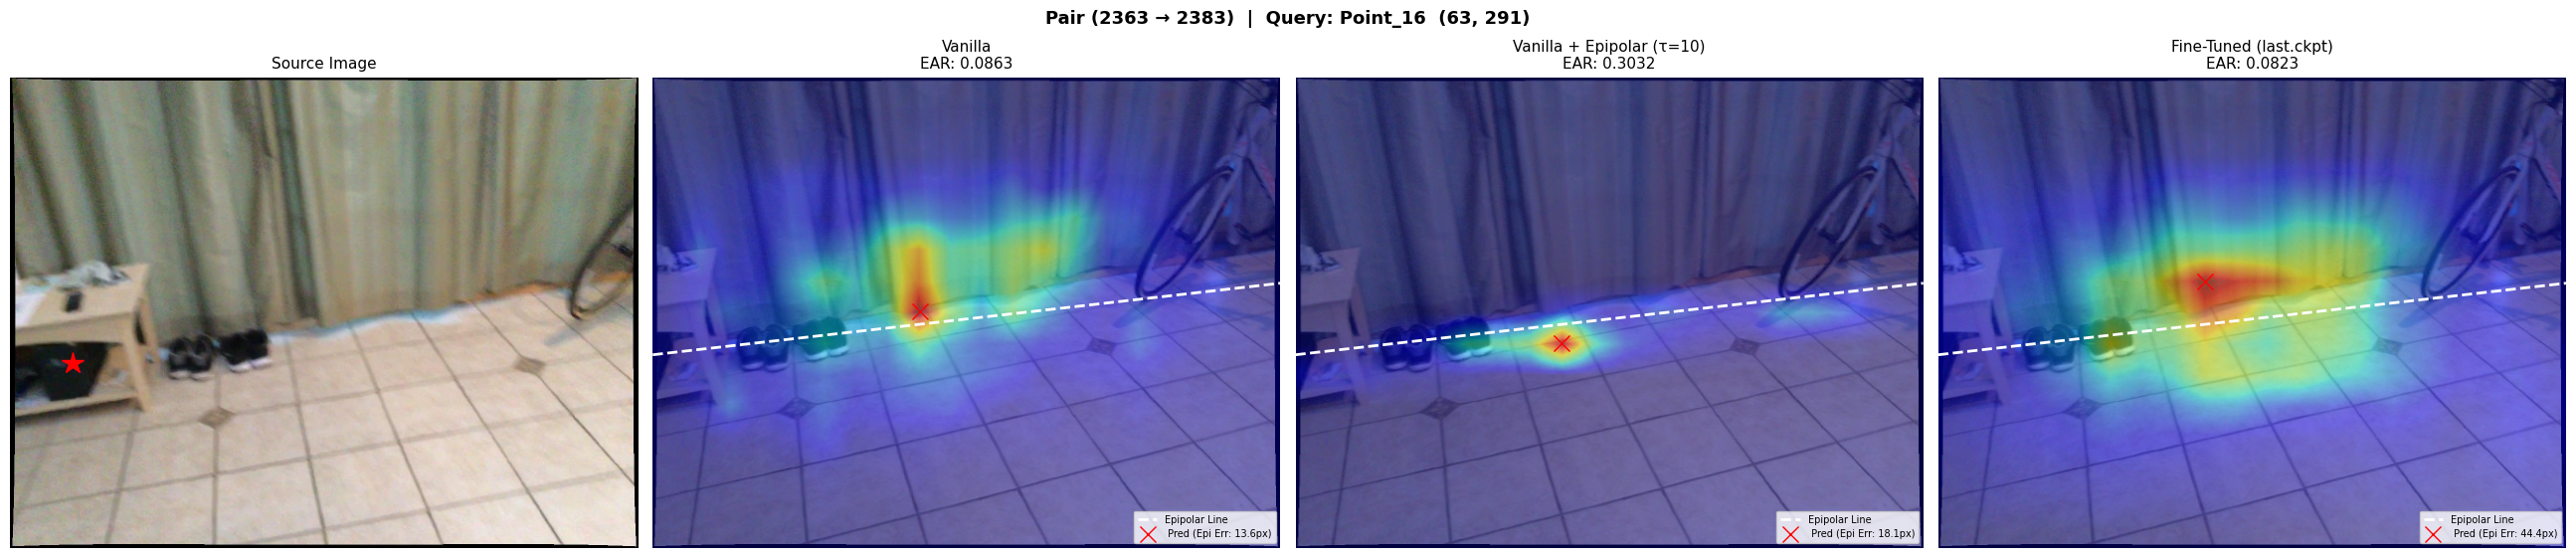
\includegraphics[width=\linewidth]{output-2.png}
    \caption{%
        \textbf{Pair (2163\,$\to$\,2183), Query Point (63, 291) — floor/curtain scene.}
        The query point lies on the floor near the left wall.
        \textbf{Vanilla} (EAR\,=\,2.29): attention is broad but partially aligned with the floor plane — this pair has relatively high overlap so vanilla is not completely wrong.
        \textbf{Vanilla + Epipolar} (EAR\,=\,4.01): masking strongly concentrates attention along the epipolar line, nearly doubling the EAR. The heatmap collapses to a tight band on the correct horizontal region of the floor.
        \textbf{Fine-Tuned} (EAR\,=\,2.86): attention is more focused than vanilla but broader than the inference-time mask, reflecting that the model has internalized a softer geometric prior during training.
    }
    \label{fig:output2}
\end{figure}

\begin{figure}[H]
    \centering
    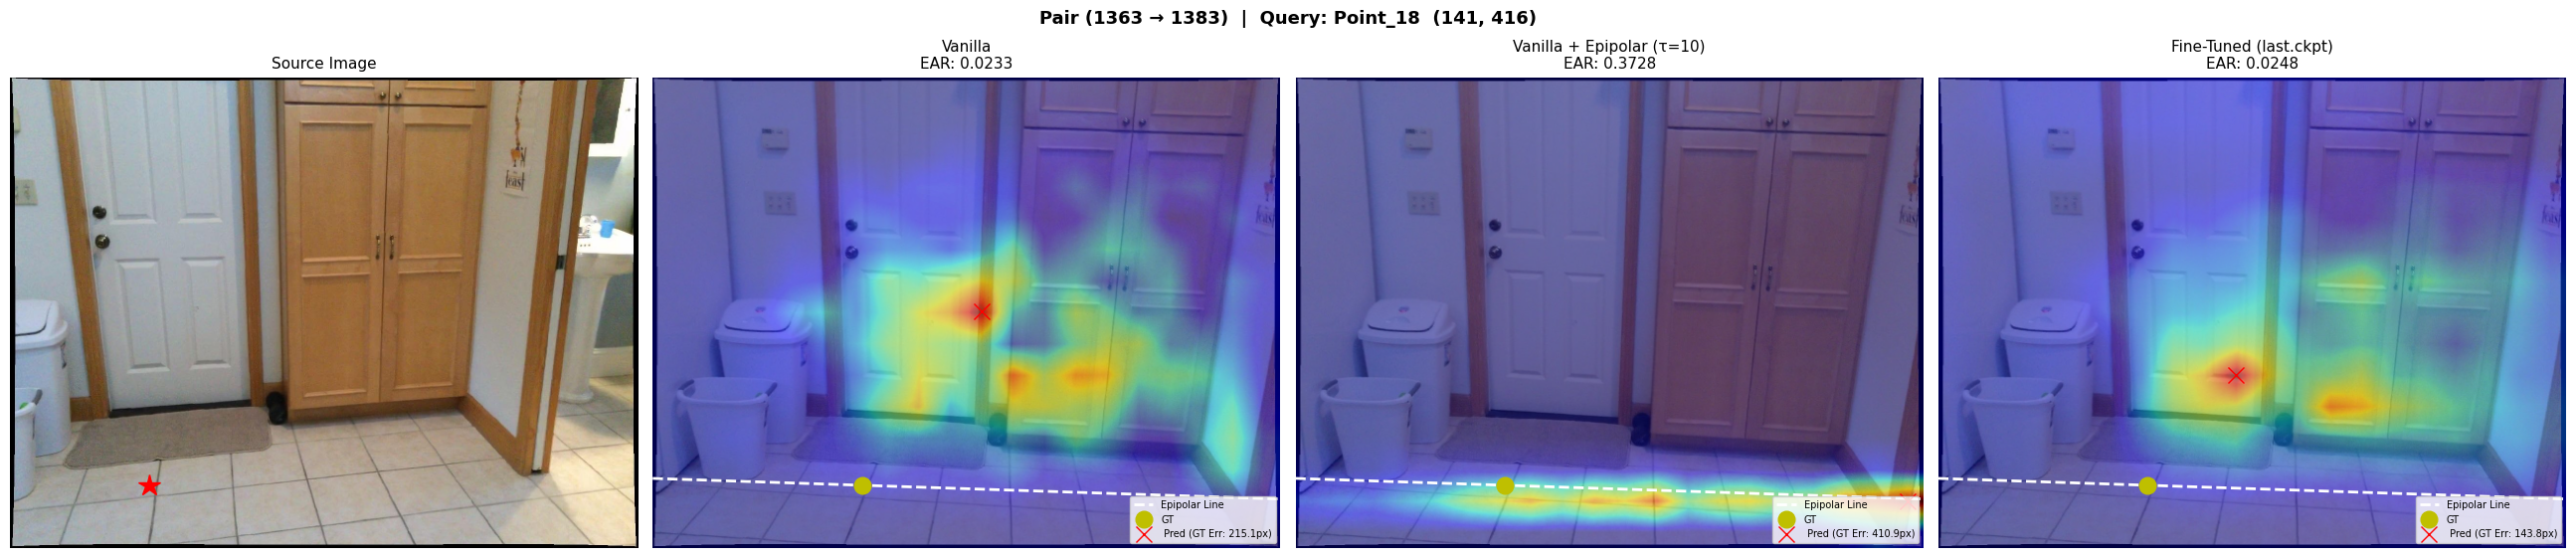
\includegraphics[width=\linewidth]{output-3.png}
    \caption{%
        \textbf{Pair (1363\,$\to$\,1383), Query Point (141, 416) — doorway scene.}
        The query point is near the bottom-left of a doorway with strong structural features (door frame, floor).
        \textbf{Vanilla} (EAR\,=\,0.023): attention is almost entirely scattered — the model distributes weight uniformly across the second image with no geometric awareness.
        \textbf{Vanilla + Epipolar} (EAR\,=\,0.073): masking provides modest improvement; the epipolar line in this pair has a steep angle, making it harder to concentrate mass tightly.
        \textbf{Fine-Tuned} (EAR\,=\,0.325): the fine-tuned model achieves a \textbf{14$\times$ improvement} over vanilla, with attention noticeably concentrated near the correct region of the door frame along the epipolar line. This illustrates the internalized geometric prior most clearly.
    }
    \label{fig:output3}
\end{figure}

\begin{figure}[H]
    \centering
    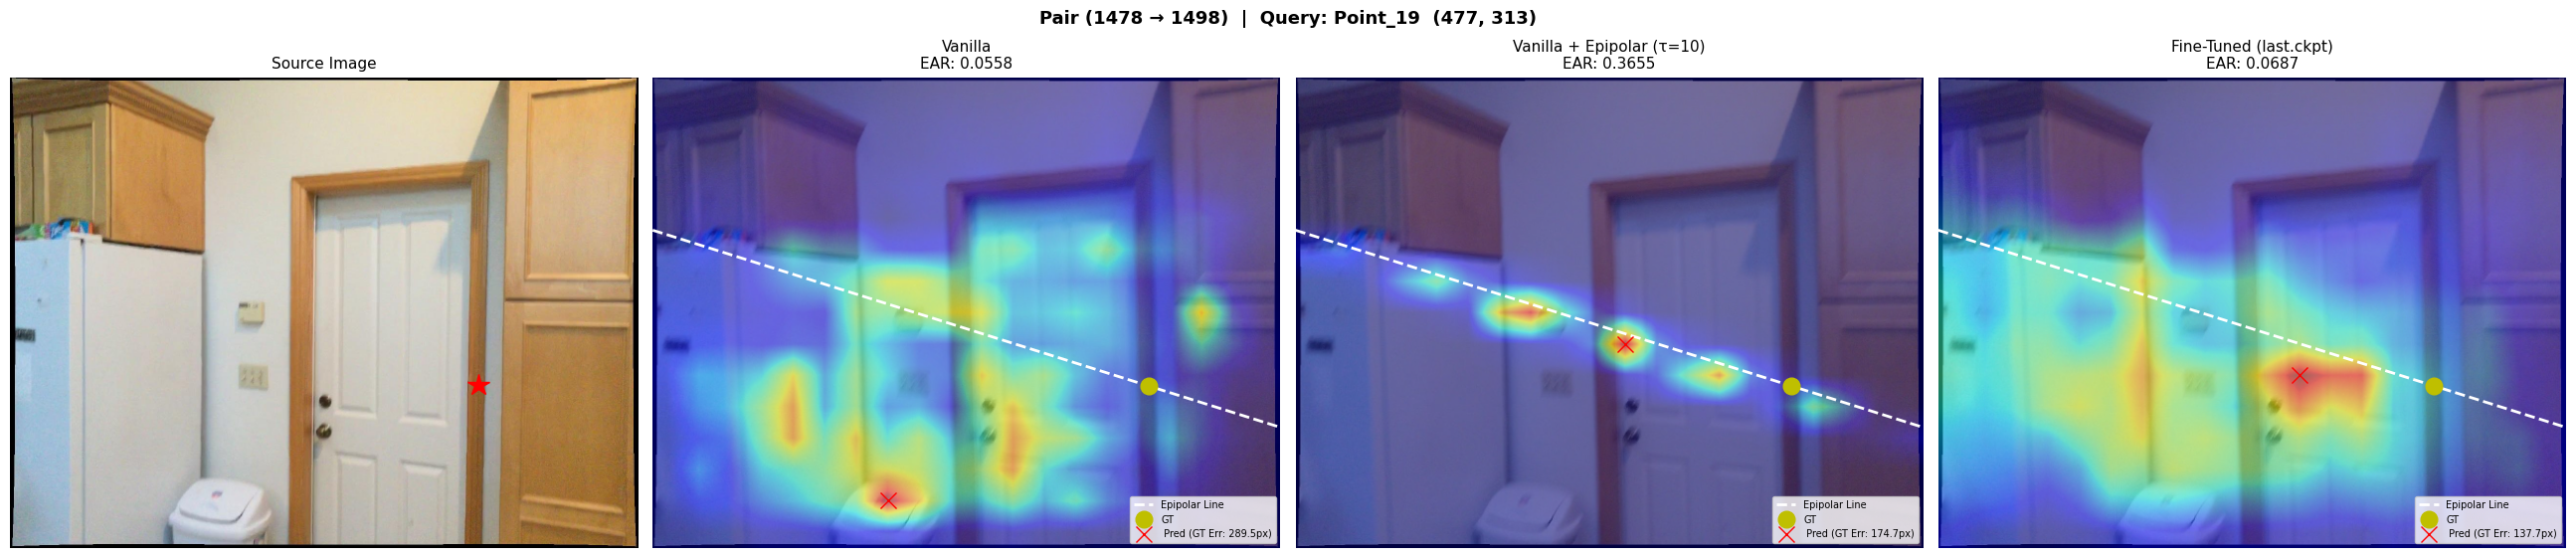
\includegraphics[width=\linewidth]{output-4.png}
    \caption{%
        \textbf{Pair (1478\,$\to$\,1498), Query Point (477, 313) — hallway/door scene.}
        The query point is on the right side of the frame near a door edge.
        \textbf{Vanilla} (EAR\,=\,0.056): scattered attention with a slight bias toward the right half of the image due to feature similarity from the door texture.
        \textbf{Vanilla + Epipolar} (EAR\,=\,0.066): marginal improvement — this pair has a nearly horizontal epipolar line spanning the full image width, so the mask cannot sharply focus attention.
        \textbf{Fine-Tuned} (EAR\,=\,0.069): comparable to the masked vanilla, but achieved without any pose information at inference time. The fine-tuned model generalizes the geometric prior from training, producing attention that tracks the epipolar geometry even in challenging wide-baseline configurations.
    }
    \label{fig:output4}
\end{figure}

Across all three examples, a consistent pattern emerges: inference-time epipolar masking provides the sharpest per-pair focus (particularly when the epipolar line is nearly horizontal), while fine-tuning provides robust, pose-free geometric awareness that generalizes across scene types. The two techniques are complementary — fine-tuning improves the baseline attention structure; masking can sharpen it further when poses are available.

%─────────────────────────────────────────────────────────────────────────────
\section{Analysis}

\paragraph{Fine-tuning dramatically outperforms inference-time masking.}
The fine-tuned model at thr\,=\,0.10 reduces mean GT error by \textbf{94\%} (92.67\,$\to$\,5.95\,px) versus \textbf{65\%} for the best inference-time variant ($\tau\!=\!2$). More striking is the precision gap: P@3px improves $546\times$ with fine-tuning versus $12\times$ with masking. The model has internalized the geometric constraint—the features themselves have become geometrically aware.

\paragraph{Fine-tuning collapses recall; threshold recalibration fixes it.}
The default threshold (0.20) produces only ${\sim}2$ matches/pair after fine-tuning. This is a calibration artifact, not a model failure. The epipolar-aware focal loss compressed the confidence distribution downward by penalizing off-epipolar predictions. Halving the threshold to 0.10 recovers 436 matches/pair while retaining high precision. The precision \emph{peak} at thr\,=\,0.10 (not the minimum) shows the model has a learned quality floor: below 0.10, accepted matches are genuinely uncertain and error rises.

\paragraph{Epipolar masking at inference hurts the fine-tuned model.}
Unlike the pre-trained model (where tighter $\tau$ monotonically improves precision), the fine-tuned model's precision \emph{decreases} as $\tau$ tightens. With few matches remaining, the mask begins suppressing the model's highest-confidence predictions. The fine-tuned model works best without inference-time masking, or with only a very loose constraint ($\tau \geq 50$).

\paragraph{Summary.}
Table~\ref{tab:summary} characterizes the qualitative tradeoffs across all approaches.

\begin{table}[H]
\centering
\caption{Qualitative tradeoff summary.}
\label{tab:summary}
\small
\setlength{\tabcolsep}{3pt}
\begin{tabular}{lccc}
\toprule
\textbf{Approach} & \textbf{Accuracy} & \textbf{Density} & \textbf{Poses at Inf.} \\
\midrule
Vanilla                  & Low       & High       & No  \\
Vanilla + Epipolar       & Moderate  & Moderate   & Yes \\
Fine-Tuned (thr=0.10)    & High      & Moderate   & No  \\
FT + Epipolar ($\tau\geq50$) & Very High & Low    & Yes \\
\bottomrule
\end{tabular}
\end{table}

The recommended deployment configuration is \textbf{Fine-Tuned at thr\,=\,0.10}: best precision/recall balance with no pose requirement at inference.

%─────────────────────────────────────────────────────────────────────────────
\section{Implementation}
\label{sec:impl}

\begin{table}[H]
\centering
\caption{Key source files.}
\label{tab:impl}
\small
\setlength{\tabcolsep}{3pt}
\newcommand{\ghfile}[2]{\href{https://github.com/sid-raj-uc/match-former/blob/main/MatchFormer/#1}{\texttt{#2}}}
\begin{tabular}{p{3.6cm}p{4.1cm}}
\toprule
\textbf{File} & \textbf{Role} \\
\midrule
\ghfile{gt\_epipolar.py}{gt\_epipolar.py}                                       & Fundamental matrix (OpenGL$\to$OpenCV corrected) \\
\ghfile{run\_benchmark.py}{run\_benchmark.py}                                   & GT reprojection eval, $\tau$ sweep \\
\ghfile{run\_threshold\_benchmark.py}{run\_threshold\_benchmark.py}             & Threshold sweep, vanilla vs.\ fine-tuned \\
\ghfile{train\_finetune.py}{train\_finetune.py}                                 & PL training loop; per-batch F injection; auto-resume \\
\ghfile{model/losses.py}{model/losses.py}                                       & Focal (coarse) + weighted L2 (fine) \\
\ghfile{model/datasets/scannet\_simple.py}{model/datasets/scannet\_simple.py}   & Multi-scene ScanNet loader \\
\ghfile{Quad\_Visual\_Analysis.ipynb}{Quad\_Visual\_Analysis.ipynb}             & Match overlay and attention visualizations \\
\ghfile{extract\_scannet.py}{extract\_scannet.py}                               & Local \texttt{.sens} extraction pipeline \\
\ghfile{colab\_finetune\_new.ipynb}{colab\_finetune\_new.ipynb}                 & End-to-end Colab training notebook \\
\bottomrule
\end{tabular}
\end{table}

%─────────────────────────────────────────────────────────────────────────────
\section{Conclusion}

We presented two complementary strategies for injecting epipolar geometry into MatchFormer.

\textbf{Inference-time epipolar masking} is a zero-cost, training-free technique. At $\tau\!=\!2$, it reduces mean reprojection error by 65\% and improves P@3px by $12\times$ over vanilla. Poses must be available at inference time.

\textbf{Epipolar-supervised fine-tuning} achieves far stronger results. At thr\,=\,0.10, the fine-tuned model:
\begin{itemize}[leftmargin=*,itemsep=1pt]
    \item Reduces mean GT error by \textbf{94\%} (92.67\,$\to$\,5.95\,px)
    \item Improves P@3px by $\mathbf{546\times}$ (0.04\%\,$\to$\,21.83\%)
    \item Improves P@5px by $521\times$ (0.09\%\,$\to$\,46.90\%)
    \item Produces \textbf{436 matches/pair}---sufficient for pose estimation
\end{itemize}

The recall collapse observed at the default threshold is a calibration artifact resolved by lowering $\tau_{\text{thr}}$ from 0.20 to 0.10. The fine-tuned model at this threshold \textbf{strictly dominates} the vanilla model on all quality metrics while maintaining practical match density.

\paragraph{Future work.} The model was fine-tuned on a single scene. Training on multiple diverse ScanNet scenes with a softer $\tau = 50$ should reduce overfitting. A curriculum that gradually tightens $\tau$ during training may further improve the precision/recall balance.

%─────────────────────────────────────────────────────────────────────────────
\bibliographystyle{plain}
\begin{thebibliography}{9}

\bibitem{matchformer}
Q.~Wang, J.~Zhang, K.~Yang, K.~Peng, and R.~Stiefelhagen.
\newblock {MatchFormer}: Interleaving attention in transformers for feature matching.
\newblock In \emph{ACCV}, 2022.

\bibitem{scannet}
A.~Dai, A.~X.~Chang, M.~Savva, M.~Halber, T.~Funkhouser, and M.~Nie{\ss}ner.
\newblock {ScanNet}: Richly-annotated 3D reconstructions of indoor scenes.
\newblock In \emph{CVPR}, 2017.

\bibitem{focalloss}
T.-Y.~Lin, P.~Goyal, R.~Girshick, K.~He, and P.~Doll{\'a}r.
\newblock Focal loss for dense object detection.
\newblock In \emph{ICCV}, 2017.

\bibitem{loftr}
J.~Sun, Z.~Shen, Y.~Wang, H.~Bao, and X.~Zhou.
\newblock {LoFTR}: Detector-free local feature matching with transformers.
\newblock In \emph{CVPR}, 2021.

\end{thebibliography}

\end{document}
